\h\ is the dominant contribution to opacity in the solar atmosphere for photons in the infrared (with wavelength $\lambda \gtrsim 1.6 \mu$m), optical, and ultraviolet regimes; since the solar luminosity peaks in this wavelength range \h\ opacity affects a significant portion of the light coming from the sun.

\cite{wishart1979} calculates the bound-free photoionization
cross-section of \h\ using close-coupling plus correlation
wavefunctions as a function of photon
over the wavelength range 1250-16300 $\AA$.  The cross-sections given
in that reference are accurate to within 1\%.
The calculated cross sections are shown as the points in
figure~\ref{fig:bfcrosssection}; the lines connecting the points are a
cubic spline interpolation.  The right side of the figure shows the
cross-section for photons with energies close to the $0.75$ eV
sufficient to ``ionize'' the \h ion to become H.  The cross-section
peaks at $\sim 8500$\AA and then decreases with increasing photon
energy.  It is interesting to note that this cross-section peaks in
the optical with large values in the near infrared and near
ultraviolet, just as does solar spectrum.  Hence, the \h\ opacity is
most relevant is the regime of photon energies where the sun's own
photon production peaks.  This coincidence causes the \h\ opacity to
be even more dominant in the sun than in stars with a similar \h\
density in their atmospheres but with a photon energy spectrum peaking
outside the optical.
\begin{figure}
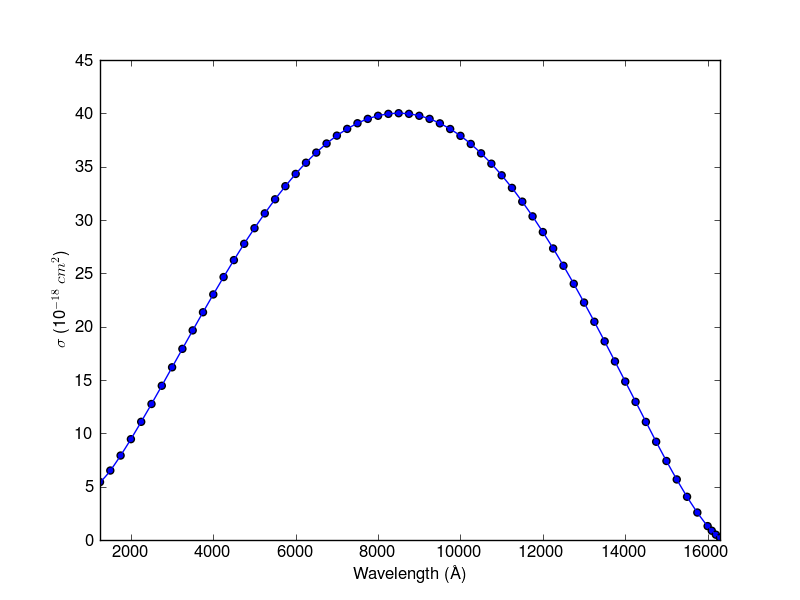
\includegraphics[width=80mm]{figs/boundfree_crosssection.png}
\caption{\label{fig:bfcrosssection}The bound-free photoionization
cross-section of \h. Tabulated values calculated
by \cite{wishart1979} are given as open circles with a cubic spline
interpolation shown as the line connecting the points.  The calculated
cross-sections span from near infrared (at the wavelengths where photon
energies are sufficiently high to ionize the least bound electron
of \h) to near ultraviolet. As shown, photon energy increases along
the x-axis from right to left.}
\end{figure}

Figure~\ref{fig:bohmopacity} shows  opacity as a function of wavelength over the range of wavelengths where \h\ bound-free opacities are relevant for a theoretical solar-like star.  At high wavelengths, past the $\sim 1.6 \mu$m cutoff for \h\ opacity free-free interactions with \h\ dominate the opacity (the H in the figure is a typo, it should be \h), while at lower wavelengths Balmer bound-free absorption begins to dominate the opacity.
\begin{figure}
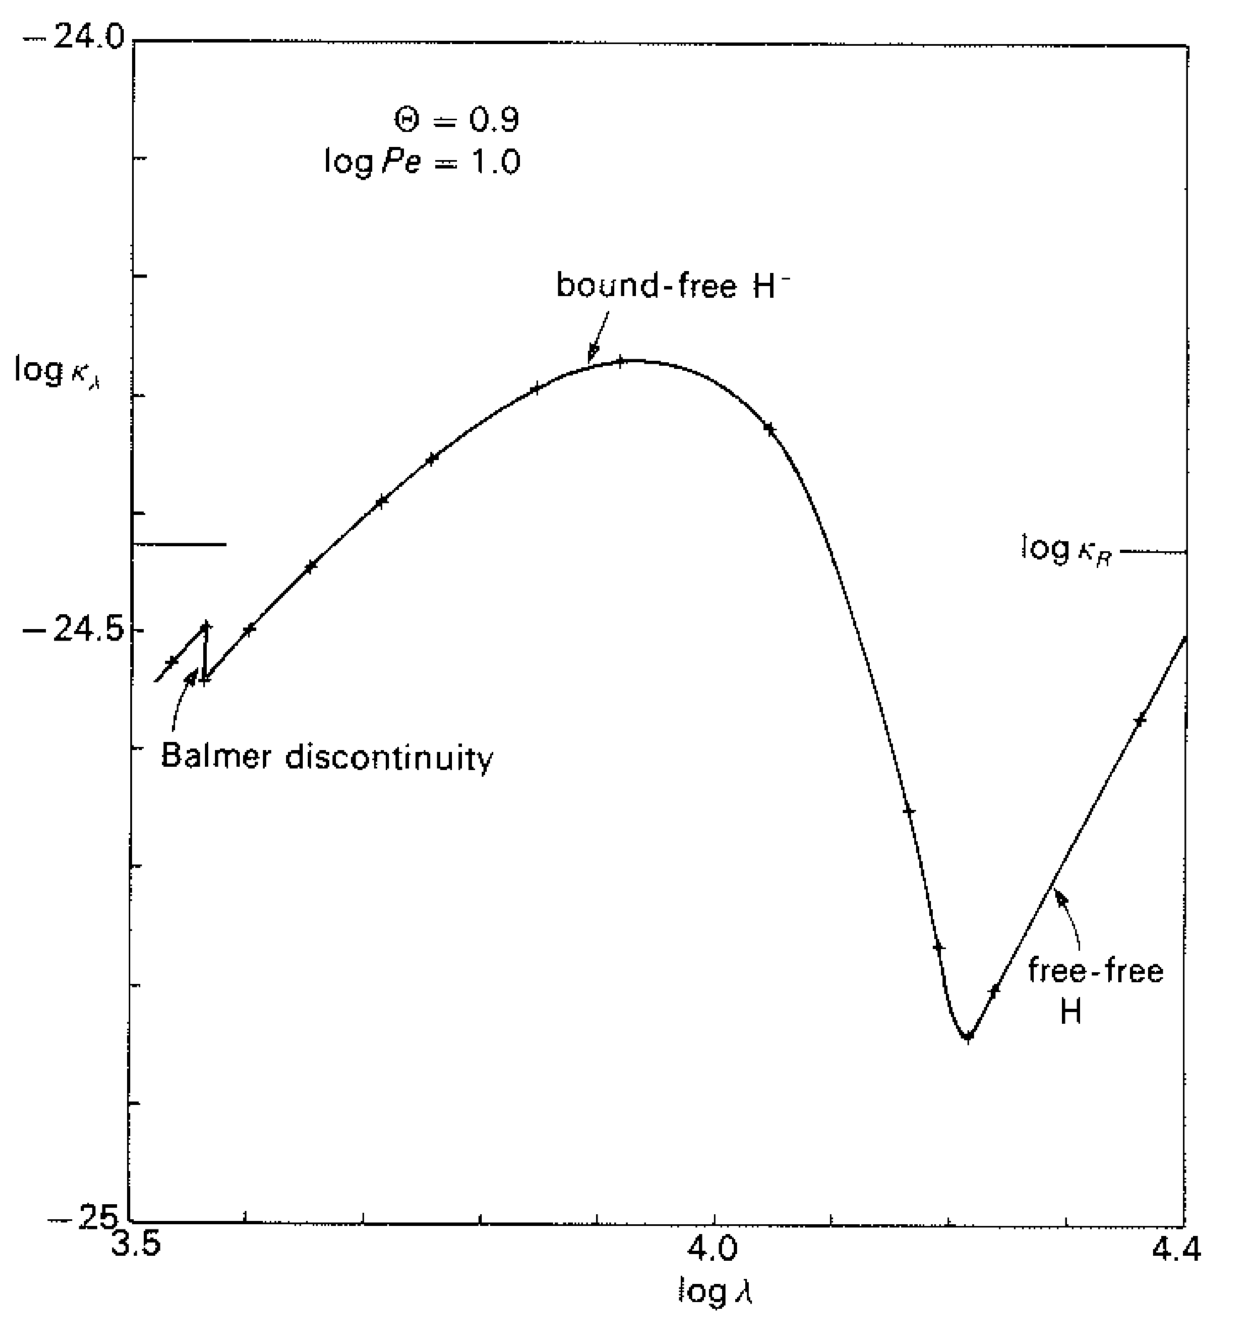
\includegraphics[width=80mm]{figs/hminusopacity.png}
\caption{\label{fig:bohmopacity}Continuous absorption coefficient per heavy particle, shown for $\Theta=0.9$ (which means $T=5600$ K and log $P_e=1.0$.  Note that the free-free contribution is mislabelled; it should be free-free from \h\ not H.  Figure from \cite{boehm1989}.}
\end{figure}

Figures~\ref{fig:bfcrosssection} and \ref{fig:bohmopacity} both show that the opacity doesn't show a discontinuity at the $\sim$1.6$\mu$m cutoff value for \h\ ``ionization'' as would be expected and is indeed seen for other species being ionized.  Figure~\ref{fig:bethe} (taken from \citealt{bethe1977}) shows $\sigma$ as a function of photon frequency relative to the frequency corresponding to the ionization energy $\nu$ for H, He, and \h.  H and He both show a large cross-section right at the threshold frequency which decays with increasing frequency; \h, however, shows a small cross-section right at the threshold which increases and reaches a maximum at $\nu/\nu_{thr}\sim$1.7.  \cite{rau1996} explains this in terms of basic quantum mechanics and angular momentum.  After a photon is absorbed by \h\ the electron departs in a $p$-wave.  In the ground state of \h, however, both the electrons are in the $s$ orbital.  Thus there is an angular momentum barrier that must be overcome, via quantum tunnelling.  Just above the ionization threshold electrons have low energy and see the angular momentum barrier as the longest range potential; the probabilities associated with tunnelling through this barrier thus affect the cross-section at these low energies. .  {\bf Can talk about Wigner 1948 E to the l+1/2 if you want. Rau page 116}.  This is not the case for neutral atoms, where the Coulomb potential is the longest-range potential.  This potential has no dependence on angular momentum and, as such, there is no angular dependence on the cross-section.
\begin{figure}
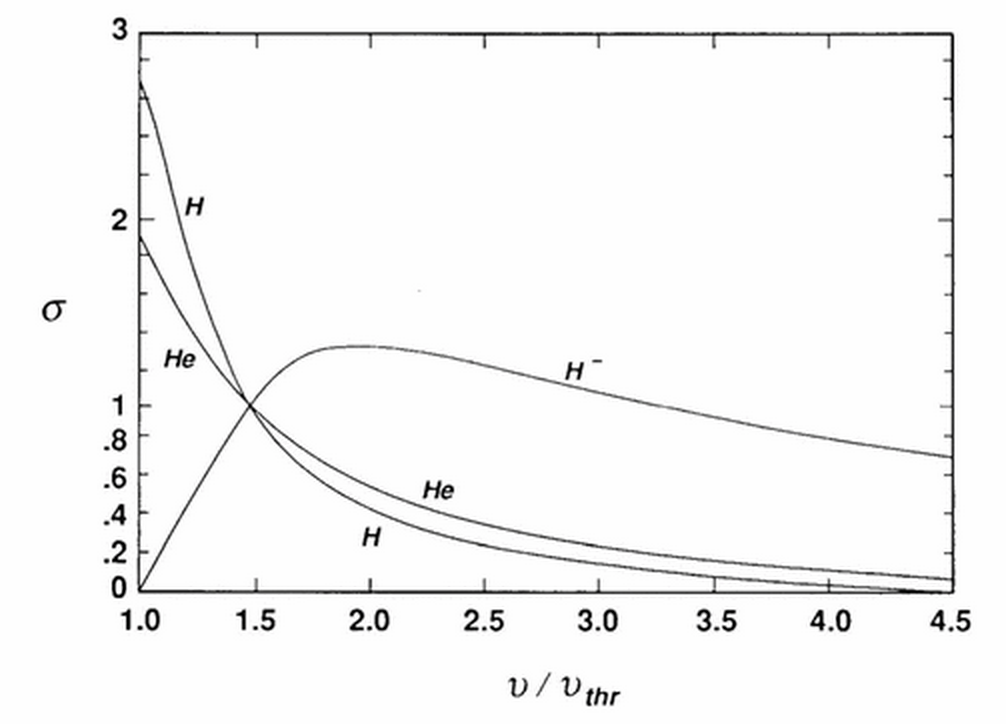
\includegraphics[width=80mm]{figs/betheplot.png}
\caption{\label{fig:bethe}Photoionization cross-section as a function of photon frequency, expressed in the unitless ratio $\nu/\nu_{thr}$, which is the ratio of the photon frequency relative to frequency of a photon with energy corresponding to the ionization energy of the species.  Cross-sections for H, He, and \h\ are shown (from \citealt{bethe1977}).}
\end{figure}

To quantify the amount of \h\ in the solar atmosphere relative to other species (and thus quantitatively understand why \h\ is the dominant opacity source) we must use the Saha ionization equation, given by
\begin{multline}
\frac{n_{i+1}}{n_i} = \frac{1}{n_e}\frac{(2\pi m_e kT)^{1.5}}{h^3}2\frac{g_{i+1}}{g_i}e^{-\chi_i/kT} \\ \approxeq \frac{2.413\times10^{15}}{n_e}T^{1.5}\times 2\frac{g_{i+1}}{g_i}e^{-\chi_i/kT}~[\textrm{cm}^{-3}\textrm{K}^{-1.5}]
\end{multline}
where $n_i$ is the number density of a species in the $i$-th ionzation state, $n_{i+1}$ is the number density of a species in the $i+1$-th ionziation state, $k$ is the Boltzmann constant, $T$ is the temperature, $h$ is the Boltmann constant, $g_i$ is the statiscal weight of the $i$-th ionzation state, $g_{i+1}$ is the corresponding quantity for the $i+1$-th ionziation state, and $\chi_i$ is the energy associated with moving from the $i$-th state to the $i+1$-th state.  A very important consideration for using the Saha equation, especially in the case of calculating \h\ abundances, is finding the quantity $n_e$, the number density of free electrons, since in atmospheres of mixed species (which describes all stellar atmospheres) all species can contribute electrons to the overall $n_e$.  In the sun, electrons contributed from H, He, and metals must all be considered in calculating $n_e$.

